\documentclass[10pt,conference,compsocconf]{IEEEtran}

\usepackage{./packages_macros}
\newacronym{ML}{ML}{machine learning}

\begin{document}
\title{Higgs Boson Machine Learning Project}

\author{
  Maryam Zakani, Zahra Farsijani, Reza Ghanaatian\\
  \textit{Machine Learning Course - EPFL - Switzerland}
}

\maketitle

\begin{abstract}
Machine learning (ML) techniques are becoming popular because they can effectively solve problems by giving the ability of learning from data.
In this project, we study the performance of six ML algorithms by performing a binary classification on a real life data-set.
We further propose multiple methods, namely data pre-processing and feature augmentation to improve the classification performance. 
\end{abstract}

%%%%%%%%%%%%%---------------------------------------------------------------------------
\section{Introduction}

\Gls{ML} techniques have attracted attention as they become important computing tools in different scientific disciplines, specially where designing and programming explicit algorithms with good performance is difficult or infeasible. The \gls{ML} algorithms learn from a data-set and make predication on data-sets through a model. 

The Higgs Boson is an elementary particle which explains why other particles have mass. This particle was discovered in collision experiments at CERN and was announced in March 2013. Such data-sets are used to distinguish signals of the Higgs Boson from background noise by performing a binary classification.
In this project we try to use machine learning algorithms to efficiently perform the classification task.
More Specifically, we first implement six \gls{ML} methods and compare their performance in the classification problem. We then explore different approaches to optimize the classification accuracy. We finally provide the predication results for the proposed approaches.


%%%%%%%%%%%%%---------------------------------------------------------------------------
\section{Implementation of \gls{ML} Methods}\label{sec:ml}

We first implement the six \gls{ML} methods, required for this project, and test them with the provided training data-set. Table~\ref{sec:ml} summarizes the prediction results. In order to get the results, we perform both cross validation on the training data, which will be explained in the next section and we get the scores from Kaggle submissions. Further, the parameter values for the algorithms in this table are chosen with an optimization through a few trials as we are mainly interested in getting an initial result of each algorithm for the first step.
We later use grid search to find the optimum value of the hyper-parameter(s) corresponding to the method that is used in the rest of the analysis in this project.

The initial evaluation shows that Least Square and Ridge Regression algorithms achieve better prediction accuracies among others without any specific optimization being performed on them, as they have fewer parameters compared to the other algorithms. This allows us to separate the optimization of the parameters from data pre-processing and continue with these two methods for the data analysis.


\section{Data-Set Processing and Analysis}\label{sec:data}

In this section we explain different approaches that we used to process the data-set and achieve a better prediction algorithm.

\subsection{Data Pre-processing}
The first step to improve the accuracy of the \gls{ML} algorithms is to remove the outliers.
In exploring the training data-set we have found that a lot values are $-999$, which indicates the case that no data was provided. More specifically, $11$ columns from the features contain $-999$ values.
We show the \emph{box plot} of the first feature, i.e., DER\_mass\_MMC in Fig.~\ref{fig:boxplot} to better show the outliers for this feature.
This plot indicates that $-999$ is an outlier for this feature.

Therefore, our first approach is to remove all the outliers from the data sets. To this end, we try the following methodologies:
\begin{itemize}
\item Remove all columns with $-999$ ($11$ columns).
\item Remove the outlier value $-999$ from all the features and replace them with the median/min/max.
\item Remove the columns with smaller weights than the weight medians.
\end{itemize}
We then use a \gls{ML} method to learn these newly generated training sets with derive the score for the generated model, however, the prediction score does not improve. Particularly, the prediction score for Least Square becomes $71.01\%$, if we remove all columns with $-999$, which shows almost no difference in comparison with initial result of this algorithm.

By further exploring the data-sets we figure out that PRI\_jet\_num is a categorical feature, which only takes four values $0,1,2,3$. Therefore, we can employ this feature to categorize the data-sets. The distributions for the data-sets according to this feature is shown in Table~\ref{tab:jet}, which indicate a similar distribution for both of the training and test sets.
Moreover, by splitting the data-sets according to the jet number, we observe that data points with jet value $0$ and $1$ have three and seven columns with all the values being $-999$, respectively. However, the data points with jet value $2$ or $3$ do not contain $-999$, except for feature DER\_mass\_MMC.
We therefore conclude that by splitting the data points to $4$ groups according to the jet number and then further split each group to $2$ subgroups, i.e., with/without the feature DER\_mass\_MMC, all the outliers can be effectively removed. We adopt this methodology for both the training and the test sets, which gives an accuracy improvement of $2\%$ for the first splitting and $0.6\%$ for the second splitting.
 

\subsection{Feature Augmentation}
In order to improve the prediction accuracy, we augment the features by several methodologies.
First, we add different power of the features as new set of features. More specifically, we add power of $2$, $3$, etc of the features. The augmented features can improve the prediction accuracy up to $80\%$ on the training set, however, they fail to improve the accuracy on the test set due to over-fitting. Therefore, we do not use this augmentation for the final training.

We further add new features by computing the cross terms of the existing features for each group of data. Unfortunately, we could not test this augmentation methodology because of time constraint as adding the cross terms will heavily increase the size of the data-set and the processing time.\footnote{Assuming that the dimension of the features is $30$, adding a cross feature will increase it to $30+30*29=900$}

\subsection{Cross Validation}
In order to find the optimum value of the super parameters and to avoid over-fitting during the training we implement a $10$-fold cross validation mechanism.
We use the method for all the explorations on the training set and we take an average out of the $10$ results.


\begin{figure}[tbp]
	\centering
	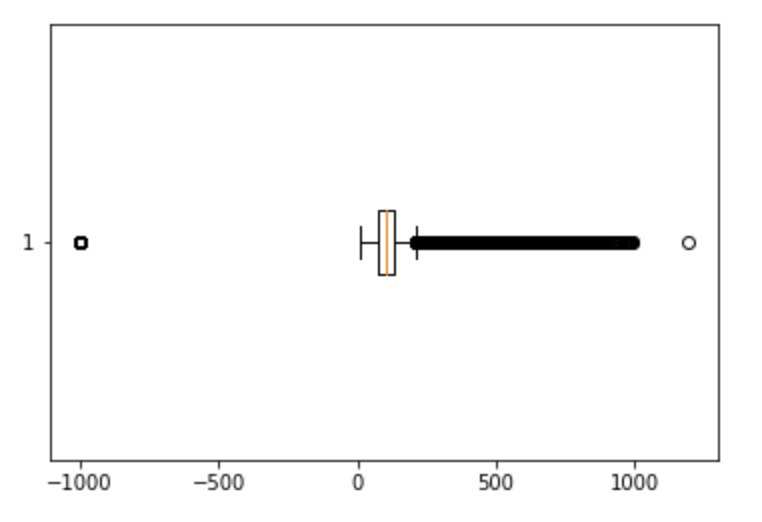
\includegraphics[width=0.7\columnwidth]{boxplot}
	\caption{Boxplot for feature DER\_mass\_MMC}
	%\vspace{-3mm}
	\label{fig:boxplot}
\end{figure}
\begin{table}[t]
	\caption{Implementation details and results for \gls{ML} methods}\label{tab:ml}
	\centering
	\resizebox{\columnwidth}{!}
	{
		\begin{tabular}{|c|c|c|c|c|c|}
			\hline
			\Xhline{2\arrayrulewidth}
			ML method & \multicolumn{3}{c|}{parameters} & \multicolumn{2}{c|}{prediction score \%} \\ [1mm]
			& $\lambda$ & $\gamma$ & max iteration & training set & test set \\ [1mm]
			\Xhline{2\arrayrulewidth} 
			Gradient Descent & -- & $0.7$ & $1$ & $50$ & $64$\\[1mm]
			Stochastic Gradient Descent & -- & $0.7$ & $10$ & $67$ & $70$\\[1mm]
			Least Square & -- & -- & -- & $74$& $74.04$\\[1mm]
			Ridge Regression & $0.001$ & -- & -- & $72$ & -- \\[1mm]
			Logistic Regression & -- & $0.3$ & $100$ & $66$ & --\\[1mm]
			Regularized Logistic Regression & $0.001$ & $0.3$ & $100$ & $67$ & --\\[1mm]
			\hline
		\end{tabular}
	}
\end{table}

\begin{table}[t]
	\caption{Distribution of the training and test data-set according to PRI\_jet\_num}\label{tab:jet}
	\centering
	%\resizebox{\columnwidth}{!}
	{
		\begin{tabular}{|c|c|c|c|c|}
			\hline
			\Xhline{2\arrayrulewidth}
			jet number & $0$ & $1$ & $2$ & $3$ \\ [1mm]
			\Xhline{2\arrayrulewidth} 
			Training set & $0.399$ & $0.310$ & $0.201$ & $0.088$ \\[1mm]
			Test set & $0.400$ & $0.308$ & $0.201$ & $0.089$ \\[1mm]
			\hline
		\end{tabular}
	}
\end{table}

%%%%%%%%%%%%%---------------------------------------------------------------------------
\section{Results}
In the previous section, we have reviewed multiple techniques to improve the classification accuracy.
We finally used the splitting technique to group the data points into $8$ categories. Further, we did not use any augmented features.
The Ridge regression algorithm is used as the learning method and the optimum $\lambda$ value for each group are found with a greed search, which avoid possible over-fitting.
Table~\ref{tab:result} shows the classification accuracy for all groups of data on the training set, using cross validation, and on the test set, from Kaggle submission.
The final prediction accuracy is then derived by weighted-averaging across all $8$ groups and is equal to \textbf{$76.3$}.


\begin{table}[t]
	\caption{Final prediction results using Ridge Regression on training and test sets while splitting the data point ans feature augmentation are employed}\label{tab:result}
	\centering
	%\resizebox{\columnwidth}{!}
	{
		\begin{tabular}{|l|c|c|c|}
			\hline
			\Xhline{2\arrayrulewidth}
			&   & \multicolumn{2}{c|}{prediction accuracy \%} \\[1mm]
			 data points & $\lambda$ & \multicolumn{1}{c|}{training set} & \multicolumn{1}{c|}{test set} \\ [1mm]
			\Xhline{2\arrayrulewidth} 
			jet $0$ with mass 	& $1\times10^{-4}$     	& $78.2$ &  \\[1mm]
			jet $0$ without mass 		& $1$  	& $94.4$ &  \\[1mm]
			jet $1$ with mass  	& $1\times10^{-6} $ 	& $69.4$ &	\\[1mm]
			jet $1$ without mass 		& $1\times10^{-4}$   	& $90.9$ & 	\\[1mm]
			jet $2$ with mass   	& $1\times10^{-3}$  	& $72.6$ &	\\[1mm]
			jet $2$ without mass 		& $0.5$     	& $88.3$ & 	\\[1mm]
			jet $3$ with mass   	& $0.01$     	& $70.5$ & 	\\[1mm]
			jet $3$ without mass 		& $0.5$     & $91.4$ & 	\\[1mm]
			\hline
			average & -- & $\textbf{76.3331}$ & $\textbf{76.409}$\\[1mm]
			\hline
		\end{tabular}
	}
\end{table}






\section{Conclusion}
In this project we have implemented several \gls{ML} methods we were requested, namely, Gradient Descent, Stochastic Gradient Descent, Least Square, Ridge Regression, Logistic Regression and Regularized Logistic Regression, and tested them on real-life data to do a binary classification.
We learned that data pre-processing is essential to improve the predication accuracy of \gls{ML} methods. The pre-processing is often data-dependent and therefore, needs to be performed with a knowledge of the features. This knowledge is mainly achieved by means of much data exploration that is performed at an early stage in a formal machine learning project such as this one.
We realized that feature augmentation can be used to improve the accuracy, although it may increase the chance of over-fitting.
Finally, using the methodologies and algorithms explained in this report, we were able to make predictions on the test set and achieve a score of 0.76409 on Kaggle.  

%\bibliographystyle{IEEEtran}
%\bibliography{literature}

\end{document}
